\documentclass[10pt]{amsart}
\usepackage{times,amsmath,amsbsy,amssymb,amscd,mathrsfs}
\usepackage{slashbox}\usepackage{booktabs,graphicx,subfigure,epstopdf,wrapfig,chemarrow}

\usepackage{algorithm2e} 
\usepackage{multicol,multirow}
\usepackage{mathtools}
\usepackage[usenames,dvipsnames,svgnames,table]{xcolor}
\usepackage[all]{xy}
\usepackage{wrapfig}
\usepackage{tcolorbox}
\usepackage{stmaryrd}
%\usepackage[labelformat=simple]{subfig}
%\usepackage[hang,small,bf]{caption}

\usepackage{tikz,tikz-cd}
\usepackage[utf8]{inputenc}
\usepackage{pgfplots} 
\usepackage{pgfgantt}
\usepackage{pdflscape}
\pgfplotsset{compat=newest} 
\pgfplotsset{plot coordinates/math parser=false}
\newlength\fwidth

%\usepackage[notcite,notref]{showkeys}
\usepackage[numbered]{mcode}

\definecolor{myBlue}{rgb}{0.0,0.0,0.55}
%\definecolor{green}{rgb}{0.0,0.7,0.2}
\usepackage[pdftex,colorlinks=true,citecolor=myBlue,linkcolor=myBlue]{hyperref}

\usepackage[hyperpageref]{backref}
\usepackage{circledsteps}

%\newcommand{\LC}[1]{\textcolor{cyan}{#1}}
\newcommand{\LC}[1]{\textcolor{red}{#1}}

\usepackage{comment,enumerate,multicol,xspace}

  \newcounter{mnote}
  \setcounter{mnote}{0}
  \newcommand{\mnote}[1]{\addtocounter{mnote}{1}
    \ensuremath{{}^{\bullet\arabic{mnote}}}
    \marginpar{\footnotesize\em\color{red}\ensuremath{\bullet\arabic{mnote}}#1}}
  \let\oldmarginpar\marginpar
    \renewcommand\marginpar[1]{\-\oldmarginpar[\raggedleft\footnotesize #1]%
    {\raggedright\footnotesize #1}}

%\usepackage[pdftex,dvipsnames]{xcolor}

%\usepackage{xargs} % Use more than one optional parameter in a new commands
%\usepackage[colorinlistoftodos,prependcaption,textsize=footnotesize]{todonotes}
%
%\newcounter{mycomment}
%\newcommand{\mycomment}[2][]{%
%% initials of the author (optional) + note in the margin
%\refstepcounter{mycomment}%
%{%
%\todo[linecolor=blue,backgroundcolor=blue!25,bordercolor=blue]{%
%\textbf{Comment [{\sc #1\themycomment}]:}\\#2}%
%}}
%
%\newcommandx{\change}[2][1=]
%{\todo[linecolor=OliveGreen,backgroundcolor=OliveGreen!25,bordercolor=OliveGreen,#1]{%
%{\sc Change}:\\#2}}
%
%\newcommandx{\improvement}[2][1=]
%{\todo[linecolor=Plum,backgroundcolor=Plum!25,bordercolor=Plum,#1]{%
%{\sc Improvement}:\\#2}}
%
%\newcommandx{\unsure}[2][1=]
%{\todo[linecolor=red,backgroundcolor=red!25,bordercolor=red,#1]{%
%{\sc Unsure}:\\ #2}}
%

% \newcommand{\mnote}[1]{}
\newcommand{\breakline}{
\begin{center}
------------------------------------------------------------------------------------------------------------
\end{center}
}
%\usepackage{geometry}
%%\usepackage{graphicx,pst-eps,epstopdf}
%\geometry{letterpaper, margin=1.5in}

\newtheorem{theorem}{Theorem}[section]
\newtheorem{lemma}[theorem]{Lemma}
\newtheorem{corollary}[theorem]{Corollary}
\newtheorem{proposition}[theorem]{Proposition}
\newtheorem{definition}[theorem]{Definition}
\newtheorem{example}[theorem]{Example}
\newtheorem{exercise}[theorem]{Exercise}
\newtheorem{question}[theorem]{Question}
\newtheorem{remark}[theorem]{Remark}
\newtheorem{alg}[theorem]{Algorithm}
%\newtheorem{answer}[proof]{Question}

\newcommand{\dx}{\,{\rm d}x}
\newcommand{\dd}{\,{\rm d}}
\newcommand{\deq}{\stackrel{\rm def}{=}}
\newcommand{\mbb}{\mathbb}
\newcommand{\mbf}{\bs}
\newcommand{\bs}{\boldsymbol}
\newcommand{\mcal}{\mathcal}
\newcommand{\mc}{\mcode}
\newcommand{\lla}{\langle}
\newcommand{\rra}{\rangle}
\newcommand{\supp}{\operatorname{supp}}
\newcommand{\range}{\operatorname{range}}
\newcommand{\PartSize}{\fontsize{0.85cm}{0.85cm}\selectfont} 
\newcommand{\mscr}{\mathscr}
\DeclarePairedDelimiter\ceil{\lceil}{\rceil}
\DeclarePairedDelimiter\floor{\lfloor}{\rfloor}

%\newcommand{\span}{\rm span}
\newcommand{\red}{\color{red}}
\newcommand{\green}{\color{green}}
\newcommand{\blue}{\color{blue}}
\newcommand{\gray}{\color{gray}}

%\DeclareMathOperator*{\curl}{curl}
\DeclareMathOperator*{\img}{img}
%\DeclareMathOperator*{\span}{span}
\DeclareMathOperator*{\diag}{diag}
\newcommand{\curl}{{\rm curl\,}}
\renewcommand{\div}{\operatorname{div}}
%\renewcommand{\grad}{\operatorname{grad}}
\newcommand{\grad}{{\rm grad\,}}
\DeclareMathOperator*{\tr}{tr}
\DeclareMathOperator*{\rot}{rot}
\DeclareMathOperator*{\var}{Var}
\DeclareMathOperator{\rank}{rank}

\newcommand{\step}[1]{\noindent\raisebox{1.5pt}[10pt][0pt]{\tiny\framebox{$#1$}}\xspace}

%\usepackage[margins]{trackchanges}
%\renewcommand{\initialsOne}{chen}

\newcommand{\dual}[1]{\left\langle {#1} \right\rangle}
\newcommand{\norm}[1]{\left\Vert#1\right\Vert}
\newcommand{\snorm}[1]{\left\vert#1\right\vert}
\newcommand{\vertiii}[1]{{\left\vert\kern-0.25ex\left\vert\kern-0.25ex\left\vert #1 
    \right\vert\kern-0.25ex\right\vert\kern-0.25ex\right\vert}}


\begin{document}
\title{ODE Solvers: Multi-Step Methods}
\author{Long Chen}\date{\today}
\begin{abstract}

\end{abstract}
\maketitle

\tableofcontents

We consider numerical methods for solving the nonlinear ODE  
\begin{equation}\label{ODE}  
y' = f(x, y),\quad y(a) = y_0,  
\end{equation}  
where $t \in \mathbb{R}$ is the independent variable, $y = y(x) \in \mathbb{R}^d$ may be a vector-valued function, and the function $f(x, y)$ is given. The independent variable is change back to $x$ as the multi-step schemes is highly related to the interpolation of function $f(x)$. 

\section{Multi-Steps Methods}

\subsection{Notation}
It will be useful to introduce the following symbols representing indices, function value and derivative at various locations.

\begin{figure}[htbp]
\begin{center}
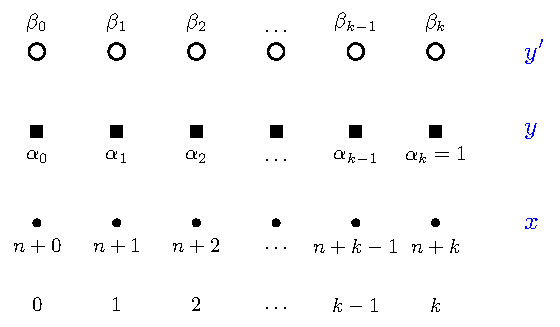
\includegraphics[width=8cm]{figures/multistep.pdf}
\caption{Notation for multi-step methods}
\label{fig:multistep}
\end{center}
\end{figure}

We use subscript to indicates the function evaluated at the corresponding grid points. For $i=0,1,\ldots, k$
$$
x_{n+i} = x_n + ih, \quad y_{n+i} = y(x_{n+i}), \quad f_{n+i} = f(x_{n+i}, y(x_{n+i})).
$$
To simply the notation and easy of analysis, we apply the change of variable  
$$
u(\hat x) = y(x_{n} + \hat xh), \quad \hat x\in [0,k] \to x = x_n+ \hat x h \in [x_n, x_{n+k}].
$$
Therefore 
\begin{equation}\label{eq:change}
u_i = y_{n+i}, \quad \dx = h \dd \hat{x}, \quad u'(\hat x) = h y'(x_{n} + \hat xh).
\end{equation}



%Depending on the context, sometimes $f_{n+i}$ could represent $f(x_{n+i}, u_{n+i})$.
\subsection{Schemes}
We can use more information on the previous steps to get a higher order methods. A general form is
\begin{equation}\label{eq:multistep}
\sum_{i=0}^k \alpha_i y_{n+i} = h\sum_{i=0}^k \beta_i f(x_{n+i}, y_{n+i}).
\end{equation}
Without loss of generality, we can assume $\alpha_k = 1$. 
\begin{enumerate}[1.]
\item $\beta_k = 0$: the scheme is explicit. 
\item $\beta_k \neq 0$: the scheme is implicit. Need to solve a nonlinear equation 
$$
y_{n+k} = ... h\beta_k f(x_{n+k}, y_{n+k}). 
$$
\end{enumerate}
In total we have $2(k+2)$ parameters, or equivalently, we know function value at $k+1$ points and its derivative at $k+1$ points, ideally we can fit a polynomial of degree $p \leq 2k+3$. 

We define residual operators by
\begin{equation}
\begin{gathered}
(R {v})(x):={v}^{\prime}(x)-{f}(x, {v}(x)), \quad {v} \in C^1[a, b], \\
(T_h)_n = \left(R_h \boldsymbol{v}\right)_n:=\frac{1}{h} \sum_{s=0}^k \alpha_s {v}_{n+s}-\sum_{s=0}^k \beta_s {f}\left(x_{n+s}, {v}_{n+s}\right), \boldsymbol{v} \in \Gamma_h[a, b].
\end{gathered}
\end{equation}

To study the truncation error, we introduce the linear operator 
$$
L u:=\sum_{s=0}^k\left[\alpha_s u(s)-\beta_s u^{\prime}(s)\right], \quad u \in C^1[\mathbb{R}] .
$$
Notice that the coordinate is changing to $\hat x\in [0,k]$ and due to the relation \eqref{eq:change}, no $h$ is in front of $u'$. 

The scheme has degree $p$ if $L u=0$ for all $u \in \mathbb{P}_p$. By linearity, this is equivalent to
\begin{equation}\label{eq:Lt}
L t^r=0, \quad r=0,1, \ldots, p
\end{equation}
Indeed we can use \eqref{eq:Lt} to determine the coefficients $(\alpha_i, \beta_i)$. For example,  we obtain the relation
$$
\begin{aligned}
p= 0: & \quad \alpha_0 + \alpha_1 = 0,\\
p= 1: & \quad \alpha_0 + \alpha_1 = 0, \alpha_0 + \beta_0 + \beta_1 = 1.
\end{aligned}
$$
Here we give several popular examples.


\subsection{Truncation error}
For ${u} \in \boldsymbol{C}^{p+1}[0, k]$, we expand $u$ by its Taylor series at $\hat x = 0$ using the Peano kernel
\begin{equation}\label{eq:Taylor}
u(\hat x) = \sum_{i=0}^p \frac{1}{i!}u^{(i)}(0) \hat x^i + \frac{1}{p!} \int_0^{\hat x} (\hat x- \sigma)^p {u}^{(p+1)}(\sigma) \mathrm{d} \sigma.
\end{equation}
By the order condition \eqref{eq:Lt}, apply $L$ to the Taylor expansion \eqref{eq:Taylor}, we get
$$
L {u}=\frac{1}{p!} \int_0^k \lambda_p(\sigma) {u}^{(p+1)}(\sigma) \mathrm{d} \sigma, \quad \lambda_p(\sigma)=L(t-\sigma)_{+}^p.
$$
Using the mean value theorem (or Lagrange remainder), we also have
$$
L {u}=\ell_{p+1} {u}^{(p+1)}(\bar{\sigma}), \quad 0<\bar{\sigma}<k ; \quad \ell_{p+1}= \frac{1}{(p+1)!} L t^{p+1}.
$$
By change of variable, we get the order of the convergence.

\begin{theorem}
A multistep method \eqref{eq:multistep} of polynomial degree $p$ has order $p$ whenever the exact solution $\boldsymbol{y}(x)$ of (6.1) is in the smoothness class $C^{p+1}[a, b]$. If the associated functional $L$ is definite, then
$$
\left({T}_h\right)_n=\ell_{p+1} {y}^{(p+1)}\left(\bar{x}_n\right) h^p, \quad x_n<\bar{x}_n<x_{n+k}
$$
where $\ell_{p+1} = \frac{1}{(p+1)!} L t^{p+1}$. Moreover, for the principal error function $\boldsymbol{\tau}$ of the method, whether definite or not, we have, if ${y} \in C^{p+2}[a, b]$,
$$
{\tau}(x)=\ell_{p+1} {y}^{(p+1)}(x).
$$
\end{theorem}

\subsection{Adams-Bashforth and Adams-Moulton methods}

\subsubsection{Adams-Bashforth method}
We take $\alpha_{k-1} = -1, \alpha_{k} = 1$ and write out the  solution $y' = f(x, y)$ as
\begin{equation}
y_{n+k} = y_{n+k-1} + \int_{x_{n+k-1}}^{x_{n+k}} y'(t)\dd t = y_{n+k-1} + \int_{x_{n+k-1}}^{x_{n+k}} f(x, y(x))\dx.
\end{equation}

Suppose we know function values $y_{n+i}$ for $i=0,\ldots, k-1$, we can evaluate to get $f_{n+i}$ and fit the data $(x_{n+i}, f_{n+i})$ with a polynomial of degree $k-1$. For example, the Lagrange interpolant $f_I$ to $f$ can be written as 
$$
p_n(f; [x_{n}, x_{n+1}, \ldots, x_{n+k-1}]; x) = \sum_{i=0}^{k-1}\ell_i(x) f_{n+i},
$$
where $\ell_i(x)\in \mathbb P_{k-1}$ and $\ell_i(x_{n+j}) = \delta_{ij}$. 

\begin{figure}[htbp]
\begin{center}
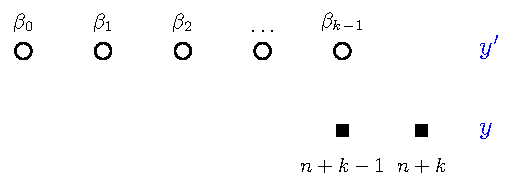
\includegraphics[width=7.5cm]{figures/ABmethod.pdf}
\caption{Adams-Bashforth method}
\label{fig:multistep}
\end{center}
\end{figure}

Approximate $f$ by $f_I$ and let $$\beta_i = \frac{1}{h}\int_{x_{n+k-1}}^{x_{n+k}} p_i(x) \dx,$$ we then obtain the Adams-Bashforth method
\begin{equation}
u_{n+k} = u_{n+k-1} + h \sum_{i=0}^{k-1}\beta_i f_{n+i}.
\end{equation}

When studying the truncation error, we assume the function value $y_{n+i}$ is known for $i=0,1,\ldots,k-1$. Then the truncation error $$T_h^{\rm AB} := \frac{1}{h} (u_{n+k} - y_{n+k}) = \frac{1}{h} \int_{x_{n+k-1}}^{x_{n+k}} (f_I - f) \dx = \frac{1}{h} \int_{x_{n+k-1}}^{x_{n+k}} ((y')_I - y') \dx.$$
We switch the integrand to $y'$ since now the remainder can be written as derivative of exact solution $y$. As the Lagrange interpolant preserves polynomial  

\subsubsection{Adams-Moulton method}
The only difference is the point $(x_{n+k}, f_{n+k})$ is included to fit the polynomial. 
\begin{figure}[htbp]
\begin{center}
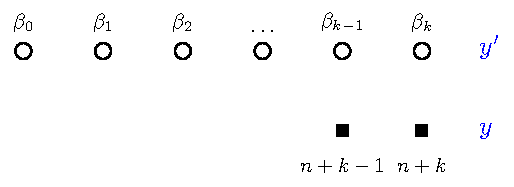
\includegraphics[width=8cm]{figures/AMmethod.pdf}
\caption{Adams-Moulton method}
\label{fig:multistep}
\end{center}
\end{figure}

Now the Lagrange interpolant $f_I$ to $f$ will be 
$$
f_I(x) = \sum_{i=0}^{k}p_i^*(x) f_{n+i},
$$
where $p_i^*(x)\in \mathbb P_{k}$ and $p_i^*(x_{n+j}) = \delta_{ij}$ for $i,j=0,1,\ldots, k$. The superscript $^*$ is introduced to distinguish the same quantity used in A-B method.

Approximate $f$ by $f_I$ and let $$\beta_i^* = \frac{1}{h}\int_{x_{n+k-1}}^{x_{n+k}} p_i^*(x) \dx,$$ we then obtain the Adams-Moultion method
\begin{equation}\label{AM}
u_{n+k} = u_{n+k-1} + h \sum_{i=0}^{k-1}\beta_i^* f_{n+i} + h\beta_k^*f(x_{n+k,} u_{n+k}).
\end{equation}
Here we single out the last term to emphasize A-M method is an implicit method and an iteration is needed to solve the nonlinear equation \eqref{AM}. 



\bibliographystyle{abbrv}
 \bibliography{/Users/longchen1/Dropbox/Math/biblib/LongLibraryZotero}
\end{document}